\documentclass[11pt,a4paper]{article}
\usepackage[margin=25mm]{geometry}
\usepackage[T1]{fontenc}
\usepackage{mathpazo,amsmath,amssymb,graphicx,booktabs,longtable,array,caption,setspace,microtype}
\usepackage[hidelinks]{hyperref}
\usepackage{fancyhdr}
\usepackage[mathlines]{lineno}
\doublespacing
\setlength{\parskip}{4pt}
\setlength{\parindent}{0pt}
\captionsetup{font=small,labelfont=bf}
\pagestyle{fancy}\fancyhf{}\fancyhead[L]{\small GBD 2023: infertility contrasts}\fancyhead[R]{\small Reproductive Health draft}\fancyfoot[C]{\thepage}
\setlength{\headheight}{14pt}
\setlength{\emergencystretch}{2em}
\newcommand{\ASPR}{\mathrm{ASPR}}
\title{Infertility subtype and reference composition in China--G20 comparisons: a GBD 2023 analysis with external survey triangulation}
\author{\parbox{0.9\textwidth}{\centering Author names, institutional addresses and corresponding author\\pending research-team completion}}
\date{25 October 2026}
\begin{document}
\maketitle
\linenumbers
\begin{abstract}
\noindent\textbf{Background:} International infertility comparisons can conceal subtype differences and changes in reference composition. We examined these issues for infertility attributed to polycystic ovarian syndrome (PCOS) and endometriosis in China, and assessed what an external population survey could corroborate.

\noindent\textbf{Methods:} We analyzed Global Burden of Disease (GBD) 2023 estimates for females aged 15--49, 1990--2023. China was compared with the other 18 sovereign G20 countries using within-age population pooling. A post hoc symmetric decomposition separated Chinese rates, reference-country rates and country population shares. An external US National Survey of Family Growth (NSFG) 2022--2023 analysis used complex-survey weights and Taylor variances. Source metadata were audited for overlap. Joint GBD draws were sought but not obtained; GBD contrasts remain point estimates.

\noindent\textbf{Results:} The negative PCOS-related infertility difference narrowed by 151.54 per 100,000. Chinese rate changes contributed +271.51, reference-country rate changes $-208.62$, and reference composition +88.65 (58.5\% of net change). Secondary infertility accounted for 69.4\% of the signed total change. Endometriosis's total difference was $-0.20$ in 2023 versus $-8.76$ in 2022. The external survey included 4,855 women aged 20--49. Age-standardized co-occurrence of diagnosis and current fertility problems was 3.94\% (survey 95\% CI 3.31--4.68) for PCOS and 2.06\% (1.62--2.61) for endometriosis. These broader co-occurrence outcomes differed from GBD etiologic attribution. Endometriosis had a lower point estimate in diagnosed women for the narrower 12-month outcome in the married/cohabiting subgroup, illustrating dependence on definition and eligible population.

\noindent\textbf{Conclusions:} Reference composition and infertility subtype materially shaped apparent convergence. External survey evidence supported reproductive-health relevance but did not validate GBD magnitudes, subtype allocation or China--G20 trends. Aligned draws and comparable independent Chinese data remain necessary for stronger inference.
\end{abstract}

\section*{Plain English summary}
Infertility estimates are often combined into one number. This can hide differences between people who have never had a live birth and those who have had a live birth previously. Comparisons between countries can also change when some countries make up a larger share of the comparison population.

We studied estimates of infertility linked to polycystic ovarian syndrome and endometriosis among women aged 15 to 49 in China and 18 other G20 countries. China's estimate for infertility linked to polycystic ovarian syndrome increased and moved closer to the comparison estimate. Part of this movement arose because the population shares of the comparison countries changed. The combined result also concealed different patterns for the two types of infertility. For endometriosis, conclusions based on the final year differed from those based on the preceding years.

These findings show why international comparisons need more detail than a single combined number. They do not tell us whether an individual woman's chance of pregnancy changed or whether healthcare improved. The main estimates come from statistical models, and we could not calculate the full uncertainty of their comparisons. We also analyzed a separate US household survey. It linked both conditions with broader fertility difficulties, but its questions and population differed from the modeled outcome. It therefore cannot confirm the size of the international differences.

\textbf{Keywords:} infertility; polycystic ovarian syndrome; endometriosis; GBD 2023; primary infertility; secondary infertility; population composition; China; National Survey of Family Growth

\section{Background}
Infertility associated with polycystic ovarian syndrome (PCOS) and endometriosis is relevant to population reproductive health as well as individualized clinical care \cite{pcos,eshre}. Estimates attributed to these causes within the Global Burden of Disease (GBD) infertility impairment describe a different outcome from total PCOS or endometriosis prevalence. They are also distinct from lifetime infertility or infertility measured exclusively among people currently trying to conceive \cite{gbd}.

Much of the descriptive territory has already been covered. Xu and colleagues analyzed both underlying diseases and their attribution to total, primary and secondary infertility in GBD 2021 \cite{xu}. Lu and colleagues examined the same two infertility causes among women aged 15--49 in China and globally, including projections \cite{lu}. Wang and colleagues subsequently analyzed infertility causes and primary/secondary attribution using GBD 2021 and 2023 \cite{wang}. Broad trend, decomposition and prediction analyses have also appeared in this journal \cite{feng}. Liu and colleagues have now combined GBD 2023 endometriosis-related infertility estimates with a Chinese clinical series, including primary/secondary patterns and the recent rebound \cite{liu2026}. Neither a newer GBD edition, subtype stratification alone, nor adding a G20 comparison constitutes a sufficient methodological advance.

A narrower unresolved question concerns the interpretation of an aggregate international contrast. A population-pooled reference combines country rates with country population shares that may change over time, even after age standardization. A narrowing difference could therefore reflect changing Chinese rates, changing reference-country rates, or changing reference-country composition. Primary and secondary infertility may contribute differently to each component. These are separable accounting questions; they do not identify causal mechanisms.

We compared China's cause-specific infertility estimates with a fixed set of 18 other sovereign G20 countries. We quantified subtype and age contributions to changes in the contrast and added an explicit decomposition of reference composition during manuscript review. We also assessed country and endpoint dependence. Endometriosis was retained as a contrasting cause, with terminal-year instability treated as a finding requiring caution rather than evidence of sustained convergence. We subsequently added an external survey arm to assess independent reproductive-health evidence and the limits imposed by non-equivalent outcome definitions.

\section{Methods}
\subsection{Design, data and outcome definitions}
This ecological secondary analysis used GBD 2023 Results Tool downloads obtained on 25 October 2026 \cite{results}. The analysis included females aged 15--49, seven five-year age groups and annual estimates for 1990--2023. China was compared with Argentina, Australia, Brazil, Canada, France, Germany, India, Indonesia, Italy, Japan, Republic of Korea, Mexico, Russian Federation, Saudi Arabia, South Africa, T\"urkiye, United Kingdom and United States of America. These are the other sovereign country members of the G20; regional organizations were excluded. The G20 is an economically defined comparison, not a matched control population or a global benchmark.

We selected infertility impairment 198, underlying causes endometriosis (607) and PCOS (605), prevalence and years lived with disability (YLDs), and Number and Rate. Primary (220) and secondary (221) infertility were downloaded separately. Matched female populations came from the same release. Main analyses concern prevalence; YLDs, case-count decompositions, country distributions, trend models and failed forecast validation are secondary results in Additional file 1. The GBD arm used aggregate estimates. The external arm, described below, used de-identified public-use respondent records without linkage to identifiable people.

The GBD methods appendix describes survey-based primary infertility in couples without a previous live birth who desire a child, have been in a union for at least five years, and report no contraceptive use. Secondary infertility also uses the interval since the last live birth. Heterogeneous survey and clinical definitions are harmonized within GBD; the resulting estimates should not be equated with a uniform 12-month clinical definition. Underlying-cause allocation occurs within the modeled infertility envelope \cite{gbd}. The denominator here is all females in each age group, not only couples attempting pregnancy.

A closer upstream audit is essential for interpretation. The methods appendix reports unchanged infertility-specific input sources from GBD 2021, disease-attribution parameters informed by the Australian Longitudinal Study on Women's Health (ALSWH), and use of primary/secondary infertility envelopes to split cause-specific sequelae, followed by reconciliation. Thus subtype patterns partly reflect shared model structure and are not independent direct observations of disease-specific primary and secondary infertility. ALSWH would not be an independent external validation source \cite{gbd}.

\subsection{Validation and standardization}
We required complete dimensional coverage, unique cells, consistent cause and infertility identifiers, finite non-negative values and ordered original marginal uncertainty bounds. Number divided by matching population was compared with official Rate. Annual subtype rates were reconstructed from Number and matched population; independent original Number/Rate exports for 1990 and 2023 checked this reconstruction. Primary plus secondary point estimates were required to reproduce the total. Input hashes, mappings and retrieval specifications accompany the code \cite{repository}.

We used published GBD 2023 standard-population weights reproduced to six decimals, normalized over ages 15--49 \cite{chen}. The original machine-precision IHME weight file was not retrieved. Thus, all standardized rates are restricted-age rates. With normalized age weight $w_a$, country $c$, age $a$, year $t$, infertility type $k$, modeled cases $C$ and female population $P$, rates per 100,000 were $r_{catk}=10^5 C_{catk}/P_{cat}$. The age-specific reference was formed before standardization:
\begin{equation}
 r_{Ratk}=\sum_{c\in R}s_{cat}r_{catk},\quad
 s_{cat}=\frac{P_{cat}}{\sum_{j\in R}P_{jat}},\quad
 A_{Ctk}=\sum_a w_a r_{Catk},\quad A_{Rtk}=\sum_a w_a r_{Ratk}.
\end{equation}
Here $R$ always excludes China. The country-share weights $s$ vary within age and year; the standard age weights $w$ are fixed. Rates were not constructed by averaging country standardized rates.

\subsection{Subtype and reference-composition accounting}
We calculated the signed difference $D_{tk}=A_{Ctk}-A_{Rtk}$ and ratio $A_{Ctk}/A_{Rtk}$. Because primary and secondary counts sum to total, their differences and changes also sum exactly. Their signed contributions are not attributable fractions or causal effects. Each age group's contribution is its standard weight multiplied by its age-specific difference change.

During manuscript review, we added a symmetric decomposition between start year 0 and end year $T$:
\begin{align}
 \Delta D_k &= X_k+Q_k+S_k,\\
 X_k &=\sum_a w_a(r_{CaTk}-r_{Ca0k}),\\
 Q_k &=-\sum_a w_a\sum_{c\in R}\frac{s_{ca0}+s_{caT}}{2}(r_{caTk}-r_{ca0k}),\\
 S_k &=-\sum_a w_a\sum_{c\in R}\frac{r_{ca0k}+r_{caTk}}{2}(s_{caT}-s_{ca0}).
\end{align}
$X$ is the Chinese rate component, $Q$ the reference-country rate component and $S$ the reference country-share component. The mean of the two replacement orders shares the product interaction symmetrically. Components sum exactly to the change in the standardized contrast, separately by subtype and age. A positive component moves China minus reference upward; with an initially negative contrast, it can indicate narrowing without indicating health improvement. This decomposition describes reference weighting, whereas the separate case-count decomposition concerns China's own population size and age distribution.

\subsection{Sensitivity analyses and uncertainty}
We excluded each reference country in turn, restricted ages to 20--49, and fixed within-age reference-country shares at their 1990 values. The symmetric decomposition was repeated for country exclusions, the restricted age range, periods starting in 1990 or 2010, and endpoints 2021, 2022 and 2023. Endpoint analyses were added after inspection of a terminal-year endometriosis increase; the reference-composition decomposition was added during manuscript review. Neither was externally preregistered. Fixed-share contrasts are a separate, order-specific sensitivity, not an interchangeable estimate of the symmetric share component.

We examined all 128 combinations of perturbing each unnormalized standard weight by half of its last published decimal. These deterministic rounding envelopes do not measure epidemiological uncertainty. Additional file 1 describes all secondary methods, including conditional trend intervals and forecast-validation rules.

We inspected the current Results Tool export settings, its 2023 user guide, the GBD 2023 data catalog and four existing input schemas. None of the retrieved exports contained draw columns. The catalog lists an on-request route for sequela-level results but does not establish availability of the required joint draws. An application specification was prepared; no aligned draws were obtained in this revision. Jointly aligned GBD draws across ages, countries and years therefore remain unavailable to this analysis. We therefore report derived point estimates without propagated uncertainty intervals or significance tests. Original marginal limits are preserved but not summed or treated as standard errors. Country exclusions describe reference sensitivity, not sampling uncertainty. YLDs and prevalence share inputs and are not independent replications. Python 3.12 and pinned NumPy, pandas, SciPy, statsmodels and Matplotlib dependencies were used. Code and machine-readable outputs are available in Additional file 2 and the repository \cite{repository}. Applicable GATHER items, including incomplete propagated uncertainty reporting, are mapped in Additional file 1 \cite{gather}.

\subsection{External survey triangulation and source independence}
We downloaded the NSFG 2022--2023 female respondent public-use file and official codebook, recode rules and variance documentation from CDC \cite{nsfg}. This was a post hoc external triangulation arm, not a prespecified validation sample. Of 5,586 respondents, 4,855 were aged 20--49 at interview. The CDC report's eligible count of 4,856 includes one woman who was 49 at screening and 50 at interview; her disease items were inapplicable. This difference does not affect the known-diagnosis domains.

Doctor-diagnosed PCOS and endometriosis were self-reported (variables PCOS and ENDO). Refusal, unknown and inapplicable responses were excluded separately for each diagnosis. Current fertility problems combined nonsurgical sterility, subfecundity or a long interval (FECUND categories 3--5) with 12-month infertility (INFERT=2). This reproduces the broader CDC indicator \cite{cdcreport}. We estimated diagnosis prevalence, fertility problems within diagnosis groups and their population co-occurrence. Co-occurrence was partitioned by no prior live birth versus at least one live birth. These birth-history categories were not relabeled as GBD primary/secondary infertility.

We retained all 20 variance strata and 80 nested clusters in domain estimation, using the final NSFG weights. Taylor linearization accounted for the complex design, with 60 design degrees of freedom. Direct standardization used the same GBD age weights renormalized over the six groups aged 20--49; respondent influence terms were combined before variance estimation to retain cross-age covariance. Survey intervals used a logit transformation and a $t$ critical value. They describe survey sampling uncertainty, not GBD uncertainty or nonresponse bias. An independent R \texttt{survey} implementation checked point estimates and standard errors \cite{survey}. A narrower sensitivity used INFERT=2 only among married/cohabiting women; deterministic classification limits assessed unknown diagnosis responses.

We downloaded GBD 2023 US source metadata for PCOS, endometriosis and infertility impairment. NSFG 2022--2023 was not listed in these three queried input sets. This supports held-out status for these outputs but does not establish independence from every upstream GBD covariate \cite{sources}. The survey measures broader, unadjusted co-occurrence rather than female-factor etiologic infertility; its US population cannot validate Chinese rates, G20 contrasts or temporal changes. No calibration factor or observed-to-expected validation score was calculated. Additional file 1 provides the source audit and analytical checks.

\subsection{Use of artificial intelligence}
OpenAI Codex was used for coding, execution assistance, source retrieval and manuscript drafting, including this revision. No artificial observations were substituted for the downloaded GBD data. Final human review of code, sources, interpretation and all author declarations remains necessary before submission. The tool is not an author and cannot approve the manuscript.

\section{Results}
\subsection{Coverage and overall contrasts}
The total burden export contained 36,176 rows and the population export 4,522 age--country--year cells. A further 36,176 annual subtype Number rows and 4,256 endpoint Number/Rate rows covered both causes and measures. Primary plus secondary reproduced total point estimates throughout. Reconstructed subtype endpoint rates agreed with original rates to within $1.51\times10^{-11}$ per 100,000. These checks establish extraction and arithmetic consistency, not independent validity of GBD estimates.

China's PCOS-related infertility standardized prevalence increased from 333.56 to 605.08 per 100,000, compared with 606.48 to 726.45 in the reference (Table~\ref{tab:prevalence}; Figure~\ref{fig:trends}). The difference changed from $-272.92$ to $-121.38$ and the ratio from 0.550 to 0.833. For endometriosis, rates changed from 63.70 to 53.30 in China and 66.63 to 53.51 in the reference. The 2023 total difference was $-0.20$; it was $-8.76$ in 2022. China's endometriosis estimate rose by 23.6\% in the last year, so the terminal comparison does not summarize a stable trajectory.

\begin{table}[htbp]\centering\small\setstretch{1.2}
\caption{Total infertility prevalence in China and the reference population.}\label{tab:prevalence}
\setlength{\tabcolsep}{3.5pt}
\begin{tabular}{llrrrrrr}\toprule
 & & \multicolumn{2}{c}{Cases, thousands} & \multicolumn{2}{c}{Rate per 100,000} & & \\
Cause & Year & China & Reference & China & Reference & $D$ & Ratio\\\midrule
Endometriosis & 1990 & 192.8 & 375.6 & 63.70 & 66.63 & -2.93 & 0.956 \\
Endometriosis & 2023 & 181.6 & 457.1 & 53.30 & 53.51 & -0.20 & 0.996 \\
PCOS & 1990 & 1083.3 & 3446.2 & 333.56 & 606.48 & -272.92 & 0.550 \\
PCOS & 2023 & 1866.7 & 6124.2 & 605.08 & 726.45 & -121.38 & 0.833 \\
\bottomrule
\end{tabular}
\caption*{Rates standardized within ages 15--49. Reference pools the other 18 sovereign G20 countries within age. $D$: China minus reference. All cells are modeled point estimates without propagated uncertainty.}
\end{table}

\subsection{Primary and secondary infertility}
In 2023, the PCOS primary-infertility difference was $-123.54$ per 100,000 (ratio 0.441), whereas the secondary difference was +2.16 (ratio 1.004; Table~\ref{tab:strata}; Figure~\ref{fig:strata}). Their changes since 1990 were +46.40 and +105.14, respectively, summing to +151.54. Thus secondary infertility accounted for 69.4\% of the signed total change. The share was 70.5\% ending in 2021 and 69.0\% ending in 2022. Across country exclusions and restriction to ages 20--49, the 2023 share ranged from 64.2\% to 75.4\%; fixing reference-country shares at 1990 yielded 78.1\%. The exact percentage therefore depends on reference construction, while secondary infertility remained the larger positive component in these checks.

The 2023 PCOS primary difference remained negative under every country exclusion ($-201.52$ to $-101.89$), but the secondary difference ranged from $-113.63$ to +30.72. Near parity of secondary infertility was therefore a main-reference result, not a stable sign conclusion. For endometriosis, the 2023 primary difference of $-7.94$ and secondary difference of +7.73 nearly canceled. Both subtype signs survived country exclusions in 2023, but the secondary difference was $-0.40$ in 2022. Its endpoint dependence limits the interpretation of cancellation.

\begin{table}[htbp]\centering\small\setstretch{1.2}
\caption{Primary and secondary infertility prevalence at the endpoints.}\label{tab:strata}
\setlength{\tabcolsep}{4pt}
\begin{tabular}{lllrrrr}\toprule
Cause & Type & Year & China rate & Ref. rate & $D$ & Ratio\\\midrule
Endometriosis & Primary & 1990 & 4.92 & 19.64 & -14.72 & 0.250 \\
Endometriosis & Primary & 2023 & 4.94 & 12.87 & -7.94 & 0.384 \\
Endometriosis & Secondary & 1990 & 58.78 & 46.98 & 11.79 & 1.251 \\
Endometriosis & Secondary & 2023 & 48.37 & 40.63 & 7.73 & 1.190 \\
PCOS & Primary & 1990 & 44.70 & 214.64 & -169.94 & 0.208 \\
PCOS & Primary & 2023 & 97.35 & 220.89 & -123.54 & 0.441 \\
PCOS & Secondary & 1990 & 288.86 & 391.84 & -102.98 & 0.737 \\
PCOS & Secondary & 2023 & 507.72 & 505.56 & 2.16 & 1.004 \\
\bottomrule
\end{tabular}
\caption*{Rate units: per 100,000 females; standardization restricted to ages 15--49. Point estimates only. Annual rates were reconstructed from Number and same-release population, with original endpoint Rate checks. Types sum to total before displayed rounding.}
\end{table}

\subsection{Changing reference composition}
For PCOS, Chinese rate changes contributed +271.51 per 100,000 to the changing contrast, reference-country rate changes $-208.62$, and reference-country share changes +88.65 (Table~\ref{tab:composition}; Figure~\ref{fig:composition}). The share component accounted for 58.5\% of the +151.54 signed net change; the combined rate components accounted for +62.89. The corresponding share components were +88.11 ending in 2021 and +86.74 ending in 2022. Across country exclusions and the age-range sensitivity, the 2023 composition share ranged from 39.8\% to 67.9\%. A material reference-composition contribution persisted, although a majority contribution did not hold in every specification.

For primary PCOS infertility, the three components were +52.65, $-38.09$ and +31.84; for secondary infertility, they were +218.86, $-170.53$ and +56.81. Thus subtype and reference composition are intersecting dimensions of the same contrast change: the 69.4\% subtype share and 58.5\% composition share must not be added. Fixing all reference-country shares at 1990 instead yielded a 2023 total difference of $-202.48$, compared with $-121.38$ under current pooling. This fixed-share calculation follows one replacement path and therefore differs from the symmetric component.

Endometriosis's +2.73 net difference change combined Chinese rate changes of $-10.39$, reference-country rate changes of +13.50 and reference composition of $-0.38$. Its near-zero net change makes percentage contributions unstable; we report absolute components. Age-by-type component tables for each endpoint accompany Additional file 2.

\begin{table}[htbp]\centering\small\setstretch{1.2}
\caption{Symmetric decomposition of changes in standardized differences, 1990--2023.}\label{tab:composition}
\setlength{\tabcolsep}{3pt}
\begin{tabular}{llrrrr}\toprule
Cause & Type & Net change & China rates & Ref. rates & Ref. shares\\\midrule
Endometriosis & Primary & +6.79 & +0.02 & +6.69 & +0.08 \\
Endometriosis & Secondary & -4.06 & -10.41 & +6.81 & -0.46 \\
Endometriosis & Total & +2.73 & -10.39 & +13.50 & -0.38 \\
PCOS & Primary & +46.40 & +52.65 & -38.09 & +31.84 \\
PCOS & Secondary & +105.14 & +218.86 & -170.53 & +56.81 \\
PCOS & Total & +151.54 & +271.51 & -208.62 & +88.65 \\
\bottomrule
\end{tabular}
\caption*{All components use per 100,000 females and sum to net change. Reference shares are country population shares within each age. Positive values move China minus reference upward. Percentages of a signed net change are accounting summaries, not causal fractions.}
\end{table}

\subsection{Age patterns and secondary analyses}
Ages 35--39 and 40--44 contributed +31.07 and +33.60 per 100,000, respectively, to the PCOS difference change, together 42.7\% of the total. These are standard-weighted contrast contributions, not case counts. The age-by-type table separates Chinese rates, reference rates and reference composition within each cell.

China's PCOS-related infertility count rose by 783,425. A separate case-count decomposition assigned +860,721 to age-specific prevalence, offset by $-68,426$ from female population size and $-8,869$ from age distribution within ages 15--49. This is consistent with increasing modeled prevalence despite demographic offsets; it does not identify its causes. The total PCOS difference remained negative across reference exclusions. The endometriosis total difference changed sign across country exclusions. Rounding the published standard weights within their evaluated precision did not reverse the main 2023 signs. Secondary YLD, trend and benchmark results are retained in Additional file 1. Forecast candidates failed the comparative validation rule, so no long-range forecasts are reported.

\subsection{External survey findings and their limits}
The survey domains with known diagnosis contained 4,813 women for endometriosis and 4,801 for PCOS. The six headline diagnosis and current-problem estimates reproduced the CDC report to its published precision \cite{cdcreport}. Current fertility problems affected 45.2\% of women reporting PCOS versus 17.1\% of those not reporting it; corresponding endometriosis values were 33.0\% and 18.6\% (Figure~\ref{fig:external}). These are unadjusted descriptive associations.

After direct age standardization, population co-occurrence was 3.94\% (survey 95\% CI 3.31--4.68) for PCOS and 2.06\% (1.62--2.61) for endometriosis (Table~\ref{tab:external}). The no-prior-live-birth components were 2.34\% and 1.40\%, respectively; the at-least-one-live-birth components were 1.59\% and 0.66\%. Components add within a diagnosis; the two diagnoses themselves are not mutually exclusive. All 20 survey point estimates and Taylor standard errors agreed with the independent R implementation to numerical precision.

Changing both the outcome and eligible population mattered. For 12-month infertility among married/cohabiting women, estimates were 12.6\% with PCOS versus 7.1\% without PCOS, and 6.5\% with endometriosis versus 7.7\% without endometriosis. Diagnosed groups contained only 29 and 15 infertility events, respectively, limiting precision. The positive broad endometriosis contrast did not persist under this narrower comparison. Missing-diagnosis classification limits for standardized co-occurrence were 3.90--4.15\% for PCOS and 2.04--2.30\% for endometriosis; these are sensitivity limits, not confidence intervals. These findings delimit the external evidence rather than calibrate GBD estimates.

\begin{table}[htbp]\centering\small\setstretch{1.2}
\caption{External survey co-occurrence of diagnosis and current fertility problems.}\label{tab:external}
\begin{tabular}{llrrr}\toprule
Diagnosis & Birth history & Events, $n$ & Estimate (\%) & Survey 95\% CI\\\midrule
Endometriosis & Total co-occurrence & 105 & 2.06 & (1.62, 2.61) \\
Endometriosis & No prior live birth & 65 & 1.40 & (1.02, 1.92) \\
Endometriosis & At least one live birth & 40 & 0.66 & (0.44, 0.97) \\
PCOS & Total co-occurrence & 208 & 3.94 & (3.31, 4.68) \\
PCOS & No prior live birth & 121 & 2.34 & (1.84, 2.98) \\
PCOS & At least one live birth & 87 & 1.59 & (1.26, 2.01) \\
\bottomrule
\end{tabular}
\caption*{NSFG 2022--2023; direct standardization within ages 20--49. Components use all women with known diagnosis status as their denominator within each age, rather than women in the birth-history subgroup. These are co-occurrence estimates, not GBD etiologic attribution. Events are unweighted counts; intervals use the survey design and exclude ascertainment and nonresponse bias.}
\end{table}

\section{Discussion}
The principal finding is that subtype composition and reference population composition both affect the interpretation of international infertility contrasts. China's negative PCOS-related infertility difference narrowed, but a substantial part of that change corresponded to population redistribution among reference countries. At the same time, secondary infertility accounted for most of the total contrast change, while a primary-infertility difference persisted. These results concern how an international comparison is constructed and what its summary conceals.

This is an incremental contribution to an extensively studied field. Previous work already examined these causes, their primary and secondary infertility attribution, China/global patterns and standard trend and decomposition methods \cite{xu,lu,wang,feng}. Our contribution is the joint accounting of subtype and within-age reference-country shares, with sensitivity to country inclusion and endpoint, plus an explicitly limited external population-survey assessment. The GBD-plus-clinical approach is also not new \cite{liu2026}; the added survey arm must be judged by the question it can answer, rather than its presence alone. We do not propose a new decomposition method or claim that GBD 2023 or subtype stratification alone is novel. The value is an interpretable application that changes the substantive reading of apparent convergence.

Age standardization removes changes in the chosen age weights, but it does not fix the mix of countries within an age group. When countries with different infertility rates gain or lose population share, a pooled reference can move even with unchanged country rates. The symmetric identity quantifies this component separately from the rate component and avoids assigning the entire rate--share interaction to one replacement order. The fixed-1990-share sensitivity gives a complementary contrast under a different reference definition. Neither is a preferred target rate or a causal counterfactual.

The subtype results further discourage describing narrowing as improved reproductive health. Both Chinese and reference PCOS rates increased. Secondary infertility's larger contribution does not show that individual women moved from primary to secondary infertility, nor that parity history caused the increase. The GBD categories reflect modeled estimates and survey definitions; diagnosis, fertility intentions, exposure to pregnancy, treatment and underlying disease attribution could all affect interpretation, but were not directly measured. The all-female denominator cannot estimate the risk among couples trying to conceive.

For endometriosis, the final-year near cancellation should be viewed as an unstable contrast. Independent download checks reproduced the source values, yet these checks cannot determine whether the abrupt terminal-year change reflects new evidence, model behavior or an actual epidemiological shift. Analyses ending in 2021 or 2022 gave a materially different overall picture. This unresolved source-level issue warrants investigation with independent evidence before a substantive convergence claim. Retaining the earlier endpoints and full annual trajectories makes the limitation visible.

Case-count accounting answers a different public-health question. The PCOS increase occurred despite offsets from China's reproductive-age female population size and age composition. The age-specific prevalence component includes any changes embedded in the modeled rates; calling it an epidemiological component does not isolate biological risk, diagnosis or policy. Clinical guidelines support individualized reproductive and broader health assessment \cite{pcos,eshre}; these ecological comparisons cannot select interventions, estimate treatment benefits or demonstrate service inequity. They can identify patterns that surveillance and independent studies should examine.

The external arm adds independently collected population observations, but it provides triangulation rather than validation of model-based cause attribution. The broad fertility-problem indicator was more common among diagnosed women, yet the endometriosis contrast reversed direction under the narrower outcome and different partnership universe. This is a substantive limit on external corroboration, not a result to omit. Ever-diagnosed conditions may include resolved disease. Diagnosis is self-reported and depends on access to care, and bivariate contrasts may reflect age, reproductive history and other factors. The female survey response rate was 23.4\%; weighting cannot ensure absence of selection bias \cite{nsfg}. The survey cannot establish Chinese trends or the direction of China--G20 gaps.

The upstream attribution audit further limits mechanistic interpretation. Disease-specific infertility and subtype allocation depend on ALSWH-derived parameters, shared infertility envelopes and reconciliation \cite{gbd}. Re-expressing these modeled outputs does not independently identify changing biological infertility risk or the effects of parity. External co-occurrence by birth history is informative about a different estimand, and cannot be substituted for the GBD type allocation.

The most serious limitation is unavailable joint uncertainty draws. We cannot propagate GBD uncertainty through pooling, standardization, subtype shares or the new decomposition. A 58.5\% or 69.4\% point estimate should therefore not be read as a precisely established population parameter. Country exclusions test dependence on the reference; they cannot replace draw-based intervals. Bootstrap resampling of the deliberately selected G20 countries would answer another question and would not recover GBD uncertainty. Conditional trend intervals are confined to the supplement and do not establish cross-country differences.

Other limitations include sparse or heterogeneous upstream evidence, modeled cause allocation, the distinction between impairment and disease prevalence, the economically selected comparison group, and the absence of an independent dataset with matching Chinese etiologic infertility definitions. The external US survey addresses a broader outcome and does not remove this limitation. Standard weights were available only as a rounded published reproduction. Several analyses were added after inspection, including endpoint checks and the reference-composition decomposition; their exploratory status requires transparent reporting and future corroboration. No release-to-release comparison was performed, so differences from previous publications cannot be assigned to real changes rather than GBD revision. These constraints limit the strength of inference even after formatting and numerical checks.

\section{Conclusions}
Within GBD 2023 point estimates, China's apparent convergence toward other G20 countries for PCOS-related infertility partly reflected changing reference-country population shares and concealed contrasting primary and secondary infertility patterns. Endometriosis near parity in 2023 depended strongly on the terminal year. International summaries should distinguish subtype, age and reference composition; these results require propagated uncertainty and comparable independent evidence before causal or policy conclusions. A held-out US survey adds evidence of reproductive-health relevance, while its differing definitions prevent validation of the GBD magnitudes and subtype allocation.

\section*{List of abbreviations}
AAPC, average annual percentage change; ARIMA, autoregressive integrated moving average; ASPR, age-standardized prevalence rate restricted here to ages 15--49; GATHER, Guidelines for Accurate and Transparent Health Estimates Reporting; GBD, Global Burden of Disease; G20, Group of Twenty; IHME, Institute for Health Metrics and Evaluation; NSFG, National Survey of Family Growth; MAE, mean absolute error; OLS, ordinary least squares; PCOS, polycystic ovarian syndrome; YLD, years lived with disability.

\section*{Declarations}
\subsection*{Ethics approval and consent to participate}
This study analyzed aggregated GBD estimates and de-identified NSFG public-use respondent records. There was no recruitment, contact with participants or access to identifiable individual records. The responsible authors must document the applicable institutional determination before submission. No institutional ethics approval or waiver has been invented for this draft.
\subsection*{Consent for publication}
Not applicable: the manuscript contains no individual person's data, images or identifiable details.
\subsection*{Availability of data and materials}
The derived datasets supporting the reported results and their analysis code are provided in Additional file 2 and the public GitHub repository \cite{repository}. Original GBD inputs are obtained from IHME through the Results Tool \cite{results}, subject to its data-use terms and access requirements. Exact dimensions, identifiers, download date, hashes and acquisition specifications are supplied. The original GBD CSVs are retained in the research archive; they are not included in the public additional file. NSFG public-use microdata and documentation are openly downloadable from CDC \cite{nsfg}; this study releases only aggregate survey outputs and code, without respondent-level extracts. Re-running the full source-to-result pipeline requires obtaining these IHME inputs. The repository contains version history; the submission manifest records the analysis revision. A permanent data/code archive identifier remains to be finalized before submission.
\subsection*{Competing interests}
Pending verified declarations from all human authors. An absence of competing interests has not been assumed.
\subsection*{Funding}
Pending author-provided funding sources, grant numbers and funder roles. No funding status has been assumed.
\subsection*{Authors' contributions}
Pending the actual human author list and verified individual contributions. All-author approval remains to be documented.
\subsection*{Acknowledgements}
We acknowledge the GBD data resource and the contributions of its data providers and collaborators. Any additional named acknowledgements and required permissions remain for the human authors to verify.

\section*{Additional files}
\textbf{Additional file 1 (PDF, with editable TeX source).} Supplementary methods, secondary case-count and trend analyses, endpoint checks, forecast validation, acquisition audit and GATHER reporting map; supplementary tables and figures.

\textbf{Additional file 2 (ZIP).} Machine-readable derived result tables, executable Python source, configuration, dependencies, acquisition and validation manifests, and a README specifying licensed IHME inputs needed to reproduce the analysis. No synthetic research observations, respondent-level extracts or raw licensed GBD downloads are included. External data retrieval specifications, source-overlap checks and survey replication outputs are included.
{\small\doublespacing
\begin{thebibliography}{99}
\bibitem{pcos} Teede HJ, Tay CT, Laven JJE, et al. Recommendations from the 2023 International Evidence-based Guideline for the Assessment and Management of Polycystic Ovary Syndrome. \emph{J Clin Endocrinol Metab}. 2023;108:2447--2469. \href{https://doi.org/10.1210/clinem/dgad463}{doi:10.1210/clinem/dgad463}.
\bibitem{eshre} Becker CM, Bokor A, Heikinheimo O, et al. ESHRE guideline: endometriosis. \emph{Hum Reprod Open}. 2022;2022:hoac009. \href{https://doi.org/10.1093/hropen/hoac009}{doi:10.1093/hropen/hoac009}.
\bibitem{gbd} GBD 2023 Collaborators. Burden of 375 diseases and injuries, risk-attributable burden of 88 risk factors, and healthy life expectancy in 204 countries and territories, including 660 subnational locations, 1990--2023: a systematic analysis for the Global Burden of Disease Study 2023. \emph{Lancet}. 2025. \href{https://doi.org/10.1016/S0140-6736(25)01637-X}{doi:10.1016/S0140-6736(25)01637-X}. Includes Supplementary Appendix 1, infertility methods.
\bibitem{xu} Xu Y, Jia Y, Li Q, et al. Global, regional, and national burden of endometriosis, PCOS, and unexplained infertility and their attribution to infertility, 1990--2021: Global Burden of Disease Study 2021. \emph{J Evid Based Med}. 2025;18:e70100. \href{https://doi.org/10.1111/jebm.70100}{doi:10.1111/jebm.70100}.
\bibitem{lu} Lu S, Zhang P, Qian H, Li HM. Analysis and projection of the disease burden of endometriosis and polycystic ovary syndrome-related infertility among women aged 15--49 years in China and globally from 1990 to 2021. \emph{Zhonghua Liu Xing Bing Xue Za Zhi}. 2026;47:1091--1098. In Chinese. \href{https://doi.org/10.3760/cma.j.cn112338-20250929-00691}{doi:10.3760/cma.j.cn112338-20250929-00691}.
\bibitem{wang} Wang J, Gan C, Jia Z, et al. Global estimates of infertility burden and contributions of congenital, endocrine, metabolic and infectious factors. \emph{Mol Med}. 2026;32:192. \href{https://doi.org/10.1186/s10020-026-01548-8}{doi:10.1186/s10020-026-01548-8}.
\bibitem{feng} Feng J, Wu Q, Liang Y, et al. Epidemiological characteristics of infertility, 1990--2021, and 15-year forecasts: an analysis based on the global burden of disease study 2021. \emph{Reprod Health}. 2025;22:26. \href{https://doi.org/10.1186/s12978-025-01966-7}{doi:10.1186/s12978-025-01966-7}.
\bibitem{liu2026} Liu Y, Hua S, Wang F, Zhou C, Wan G, Tang W. Endometriosis-associated infertility in China: epidemiological trends, future projection, and real-world clinical insights. \emph{Int J Womens Health}. 2026;18:622604. \href{https://doi.org/10.2147/IJWH.S622604}{doi:10.2147/IJWH.S622604}.
\bibitem{results} Institute for Health Metrics and Evaluation. GBD Results Tool. \url{https://vizhub.healthdata.org/gbd-results/}. Accessed 25 October 2026.
\bibitem{repository} PCOS research workspace. Analysis code, query manifests and derived results for GBD 2023 infertility comparisons. GitHub. \url{https://github.com/jiabao1314/PCOS}. Accessed 25 October 2026. Exact analysis revision is recorded in the accompanying submission manifest.\bibitem{chen} Chen S, Yang X, Jiang S, et al. Burden and temporal trends of female-specific cancers in China: a systematic analysis of the 2023 global burden of disease study. \emph{PLOS One}. 2026;21:e0351539. S1 Table: reproduced GBD 2023 standard population. \href{https://doi.org/10.1371/journal.pone.0351539}{doi:10.1371/journal.pone.0351539}.
\bibitem{gather} Stevens GA, Alkema L, Black RE, et al. Guidelines for Accurate and Transparent Health Estimates Reporting: the GATHER statement. \emph{PLOS Med}. 2016;13:e1002056. \href{https://doi.org/10.1371/journal.pmed.1002056}{doi:10.1371/journal.pmed.1002056}.
\bibitem{nsfg} National Center for Health Statistics. 2022--2023 National Survey of Family Growth: public-use data files, codebooks and documentation. CDC. \url{https://www.cdc.gov/nchs/nsfg/nsfg-2022-2023-puf.htm}. Accessed 25 October 2026. Includes female respondent data, recode specifications, design and variance documentation.
\bibitem{cdcreport} Nugent CN, Lochner KA. Endometriosis, polycystic ovary syndrome, and uterine fibroids in women ages 20--49: United States, 2022--2023. \emph{NCHS Health E-Stat}. 2026;(121):1--5. \href{https://doi.org/10.15620/cdc/252459}{doi:10.15620/cdc/252459}.
\bibitem{survey} Lumley T. survey: analysis of complex survey samples. R package version 4.5. 2026. \url{https://cran.r-project.org/package=survey}. Accessed 25 October 2026.
\bibitem{sources} Institute for Health Metrics and Evaluation. Global Burden of Disease Study 2023 Sources Tool. \url{https://sources.healthdata.org/collection/sources-2023}. Accessed 25 October 2026. US nonfatal PCOS, endometriosis and infertility metadata queries archived with this analysis.\end{thebibliography}
}

\section*{Figure legends}
\begin{figure}[htbp]\centering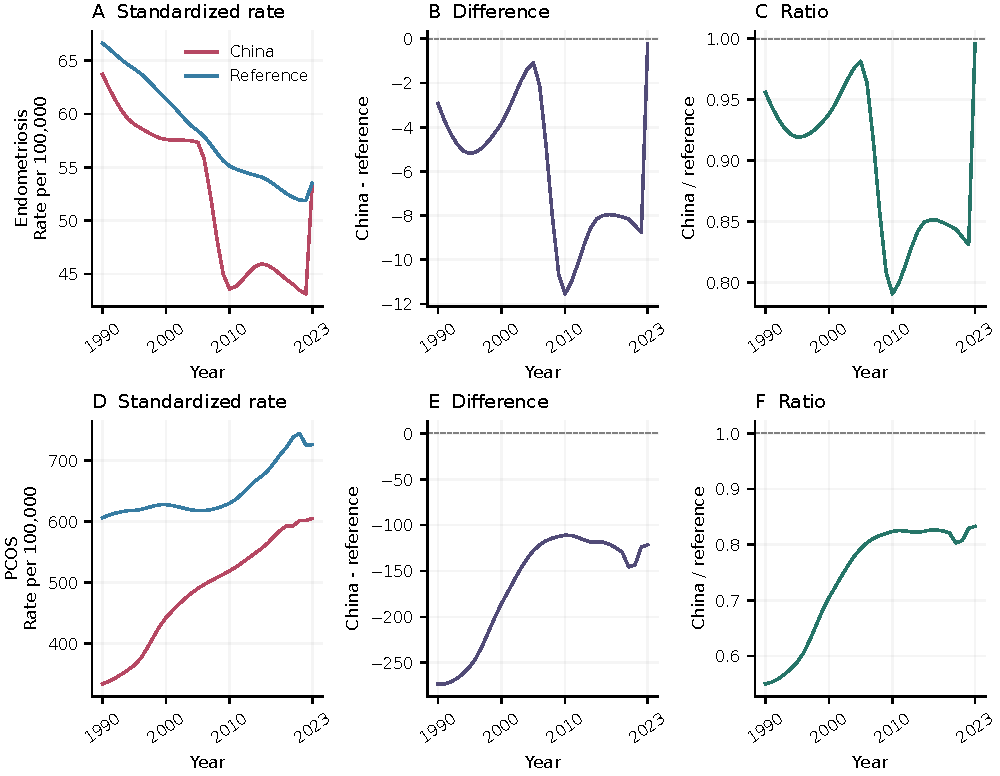
\includegraphics[width=\textwidth]{figures/RH_Figure1.pdf}
\caption{\textbf{Annual total infertility rates and China--reference contrasts.} Rates are standardized within ages 15--49. The reference pools population and modeled cases within age across 18 countries. Point trajectories have no propagated GBD uncertainty. The terminal-year endometriosis change is a source-estimate feature requiring independent corroboration.}\label{fig:trends}\end{figure}
\begin{figure}[htbp]\centering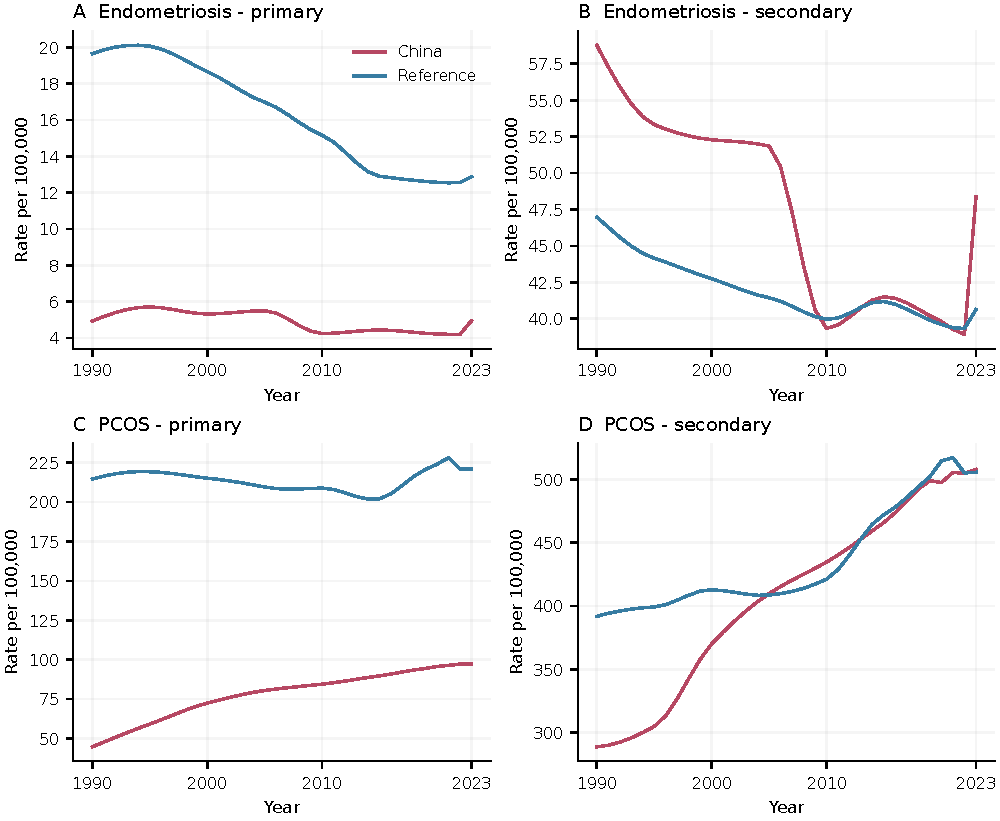
\includegraphics[width=\textwidth]{figures/RH_Figure2.pdf}
\caption{\textbf{Primary and secondary infertility trajectories.} The same restricted-age standard and annual population-pooled reference are used for both types. Opposing subtype contrasts can cancel in the total. These modeled categories do not track transitions in individual women.}\label{fig:strata}\end{figure}
\begin{figure}[htbp]\centering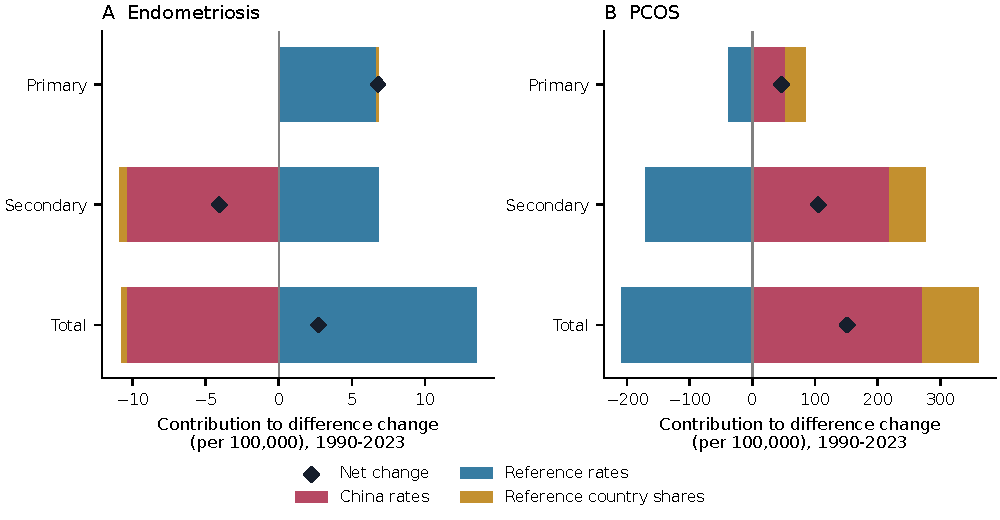
\includegraphics[width=\textwidth]{figures/RH_Figure3.pdf}
\caption{\textbf{Rate and reference-composition contributions to contrast changes.} Contributions sum to the 1990--2023 change in China minus reference, separately by infertility type. Diamonds denote net changes. Positive components move the signed contrast upward. Reference-country shares vary within age; fixed standard age weights are used throughout. The decomposition was added during manuscript review and is descriptive.}\label{fig:composition}\end{figure}
\begin{figure}[htbp]\centering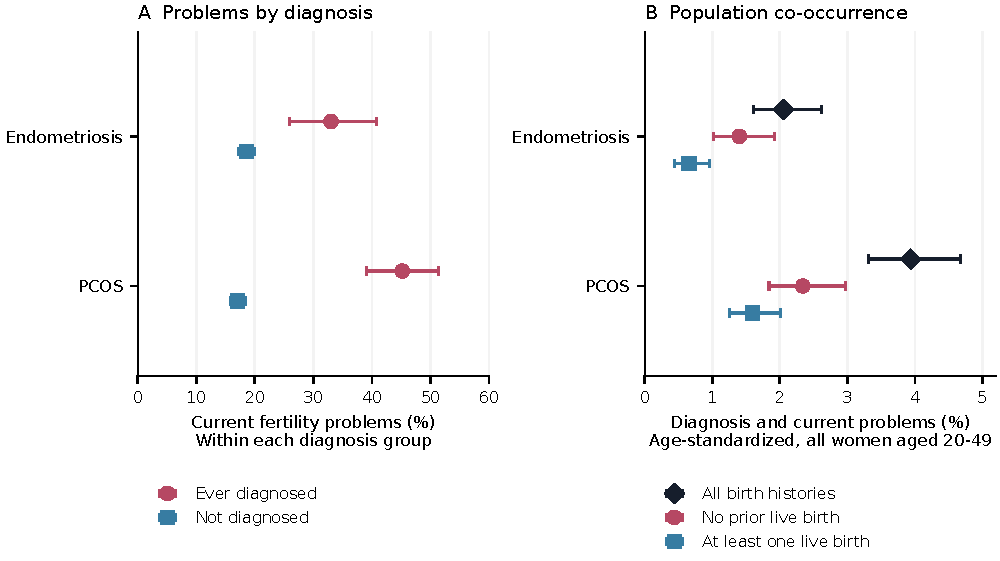
\includegraphics[width=\textwidth]{figures/RH_Figure4.pdf}
\caption{\textbf{External population-survey triangulation of reproductive-health measures.} Panel A shows crude current fertility-problem percentages within diagnosis groups. Panel B shows age-standardized co-occurrence in the population with known diagnosis status, partitioned by birth history. Error bars are survey-design 95\% intervals. Co-occurrence and birth-history groups are not GBD etiologic infertility or primary/secondary allocation. The narrower 12-month comparison gives different endometriosis results (Additional file 1).}\label{fig:external}\end{figure}
\end{document}
